\section{Ikke-konvekse strafled}
Ved at gå fra et \(\ell_2\) strafled til et \(\ell_1\) strafled, fandt vi, at for samme frihedsgrader vælger lasso en delmængde af variablerne til at have ikke-nul koefficienter og shrinks deres koefficienter mindre.
Når antallet af prediktorer er højt og antallet af relevante variable er lille, kan dette være tilstrækkeligt.
For at reducere antallet af variable tilstrækkeligt, da vil lasso måske over-shrink de valgte variable.
Derfor er det interessant at betragte ikke-konvekse strafled.

Det naturlige valg vil være \(\ell_q\) strafleddet for \(0 \leq q \leq 1\), hvor \(\ell_0\) svarer til \textit{best-subset selection}.
Figur \ref{fig:nonconvex_penalties} viser \(\ell_q\) enhedskuglerne for \(q \in \cbr{2, \ 1, \ 0.8}\)

%
\begin{figure}[H]
\centering
 \scalebox{0.5}{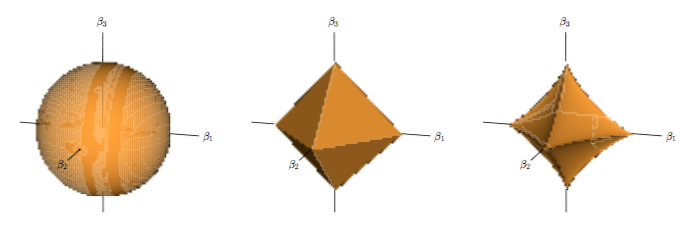
\includegraphics{fig/nonconvex_penalties.jpg}}
\caption{\(\ell_q\) enhedskuglerne i \(\mathbb{R}^3\) for \(q=2\) (venstre), \(q=1\) (midten) og \(q=0.8\) (højre). 
For \(q<1\) er betingelsesområderne ikke-konvekse. Lavere \(q\) svarer til færre ikke-nul koefficienter og mindre shrinkage.}
\label{fig:nonconvex_penalties}
\end{figure}
%

\subsection{Adaptive lasso}
\citep{adaptive_lasso} introducerede adaptive lasso som er endnu en udvidelse af standard lasso.
Ideen bag adaptive lasso er at tildele koefficienterne individuelle strafvægte istedet for at staffe koefficienterne ligeligt som i standard lasso.
Den vægtede lasso er givet ved
\begin{align*}
\arg \min_{\beta \in \R^p} \cbr{\frac{1}{2} \Vert \y - \X \beta \Vert_2^2 + \lambda \sum_{j=1}^p w_j \vert \beta_j \vert},
\end{align*}
hvor \(\mathbf{w} \in \mathbb{R}^p\) er en kendt vektor og \(w_j \geq 0\).

Adaptive lasso er blot en vægtet lasso, hvor vægtene \(\mathbf{w}\) er bestemt således at metoden opfylder orakelegenskaberne.
Lad \(\tilde{\beta}\) være et pilot estimat og definer $w_j = \frac{1}{\vert \tilde{\beta}_j \vert^\gamma}$ hvor \(\gamma>0\), da er adaptive lasso givet ved
\begin{align}
\arg \min_{\beta \in \R^p} \cbr{\frac{1}{2} \Vert \y - \X \beta \Vert_2^2 + \lambda \sum_{j=1}^p \frac{1}{\vert \tilde{\beta}_j \vert^\gamma} \vert \beta_j \vert}, \label{eq:4.76}
\end{align}
Strafleddet for adaptive lasso kan ses som en approksimation til $\ell_q$ strafleddene med $q=1-\gamma$.
Givet pilot estimaterne da er \eqref{eq:4.76} konveks.
Hvis pilot estimaterne er \(\sqrt{n}\) konsitent, da opfylder ..
Hvis \(p <n\) da kan estimaterne for mindste kvadraters metode anvendes som pilot estimater. Hvis \(p \geq n\) da er estimaterne for mindste kvadraters metode ikke defineret, men de univariate regressions koefficienter kan anvendes som pilot estimater og ...

Den aktive mængde for adaptive lasso estimatet betegnes \(\mathcal{A}_n^\text{AL} = \cbr{j \ : \hat{\beta}^{\text{AL}} \neq 0 }\)

\begin{thm}\label{thm:ALoracle}
Antag $\frac{\lambda_n}{\sqrt{n}} \rightarrow 0$ og $\lambda_n n^\frac{\gamma-1}{2} \rightarrow \infty$. Da opfylder adaptive lasso estimaterne følgende:
\begin{itemize}
\item Udvælgelsen af variabler er konsistent: $\lim_{n \rightarrow \infty} P(\mathcal{A}_n^\text{AL}=\mathcal{A})=1$
\item Asymptotisk normalitet: $\sqrt{n}\left( \hat{\boldsymbol{\beta}}_\mathcal{A}^{\text{AL}}-\boldsymbol{\beta}_\mathcal{A}^* \right) \overset{d}{\rightarrow} N(\textbf{0},\sigma^2 \boldsymbol{Q}_{11}^{-1}).$
\end{itemize} 
\end{thm}
\begin{proof}
Først bevises asymptotisk normalitet. Lad $\boldsymbol{\beta}=\boldsymbol{\beta}^{*} +\frac{\textbf{u}}{\sqrt{n}}$ og
\begin{align*}
\Psi_n(\textbf{u})=\left\Vert \mathbf{y}-\sum_{j=1}^p \textbf{x}_j \left( \beta_j^{*} +\frac{u_j}{\sqrt{n}} \right) \right\Vert^2 + \lambda_n \sum_{j=1}^p \hat{w}_j \left\vert \beta_j^{*} + \frac{u_j}{\sqrt{n}} \right\vert.
\end{align*}
Lad $\hat{\textbf{u}}^{(n)}=\arg \min \Psi_n(\textbf{u})$, da er $\hat{\boldsymbol{\beta}}^{{\text{AL}}}=\boldsymbol{\beta}^{*} + \frac{\hat{\boldsymbol{u}}^{(n)}}{\sqrt{n}}$ eller $\hat{\boldsymbol{u}}^{(n)}=\sqrt{n}\left(\hat{\boldsymbol{\beta}}^{\text{AL}}-\boldsymbol{\beta}^{*}\right)$.
Lad $V(\mathbf{u})^{(n)}=\Psi_n(\textbf{u}) - \Psi_n(\textbf{0})$, da gælder, at
\begin{align*}
V(\mathbf{u})^{(n)}= \left\Vert \textbf{y} - \sum_{j=1}^p \textbf{x}_j \left( \beta_j^{*} + \frac{u_j}{\sqrt{n}} \right) \right\Vert^2 +
\lambda_n \sum_{j=1}^p \hat{w_j} \left\vert \beta_j^{*} + \frac{u_j}{\sqrt{n}} \right\vert 
-
\left\Vert \textbf{y} - \sum_{j=1}^p \textbf{x}_j \beta_j^{*} \right\Vert^2 - \lambda_n \sum_{j=1}^p \hat{w_j} \left\vert \beta_j^{*} \right\vert.
\end{align*}
Ovenstående ligning opdeles.
Vi betragter først leddene hvori strafparametrene indgår
\begin{align*}
\lambda_n \sum_{j=1}^p \hat{w_j} \left\vert \beta_j^{*} + \frac{u_j}{\sqrt{n}} \right\vert- \lambda_n \sum_{j=1}^p \hat{w_j} \left\vert \beta_j^{*} \right\vert 
= \lambda_n \sum_{j=1}^p \hat{w_j} \left( \left\vert \beta_j^{*} + \frac{u_j}{\sqrt{n}} \right\vert - \left\vert \beta_j^{*} \right\vert
\right).
\end{align*}
Vi ser herefter på de to resterende led
\begin{align*}
\left\Vert \textbf{y} - \sum_{j=1}^p \textbf{x}_j \left( \beta_j^{*} + \frac{u_j}{\sqrt{n}} \right) \right\Vert^2 -\left\Vert \textbf{y} - \sum_{j=1}^p \textbf{x}_j \beta_j^{*} \right\Vert^2,
\end{align*}
som kan skrives på matrix-vektor form
\begin{align*}
\left\Vert \textbf{y}-\textbf{X}\boldsymbol{\beta}^{*} -\frac{\textbf{X}\textbf{u}}{\sqrt{n}} \right\Vert^2 - \left\Vert \textbf{y} - \textbf{X} \boldsymbol{\beta}^{*} \right\Vert^2  & =
\left\Vert \boldsymbol{\epsilon} - \frac{\textbf{X}\textbf{u}}{\sqrt{n}} \right\Vert^2 - \left\Vert \boldsymbol{\epsilon} \right\Vert^2  \\
&= \del{\boldsymbol{\epsilon} - \frac{\textbf{X}\textbf{u}}{\sqrt{n}}}^T \del{\boldsymbol{\epsilon} - \frac{\textbf{X}\textbf{u}}{\sqrt{n}}} - \boldsymbol{\epsilon}^T \boldsymbol{\epsilon} \\
& = \frac{\textbf{u}^T (\textbf{X}^T\textbf{X})  \textbf{u}}{n} - 2 \boldsymbol{\epsilon}^T \left( \frac{\mathbf{X}\mathbf{u}}{\sqrt{n}} \right) \\ 
&= \textbf{u}^T \left(\frac{1}{n}\textbf{X}^T\textbf{X}\right)  \textbf{u}- 2 \frac{\boldsymbol{\epsilon}^T \textbf{X}}{\sqrt{n}}\textbf{u}.
\end{align*}
Vi får så, at 
\begin{align}
V(\mathbf{u})^{(n)} & = \textbf{u}^T \left(\frac{1}{n}\textbf{X}^T\textbf{X}\right)  \textbf{u} - 2 \frac{\boldsymbol{\epsilon}^T \textbf{X}}{\sqrt{n}}\textbf{u} + \lambda_n \sum_{j=1}^p \hat{w}_j \left( \left\vert \beta_j^{*} + \frac{u_j}{\sqrt{n}} \right\vert - \left\vert \beta_j^{*}\right\vert
\right) \nonumber \\
 & = \textbf{u}^T \left(\frac{1}{n}\textbf{X}^T\textbf{X}\right)  \textbf{u} - 2 \frac{\boldsymbol{\epsilon}^T \textbf{X}}{\sqrt{n}}\textbf{u} +\frac{\lambda_n}{\sqrt{n}} \sum_{j=1}^p \hat{w}_j \sqrt{n} \left( \left\vert \beta_j^{*} + \frac{u_j}{\sqrt{n}} \right\vert - \left\vert \beta_j^{*} \right\vert
\right). \label{eq:V_4}
\end{align}
%
Af antagelse \ref{ant:tvaer}.d) har vi, at der for første led i \eqref{eq:V_4} gælder, at $\frac{1}{n} \mathbf{X}^T \mathbf{X} \overset{p}{\rightarrow} \mathbf{Q}$, mens det for andet led følger af antagelse \ref{ant:tvaer}.f), at $\frac{\boldsymbol{\epsilon}^T \mathbf{X}}{\sqrt{n}} \overset{d}{\rightarrow} \textbf{W}=N(\textbf{0},\sigma^2 \boldsymbol{Q})$. Derfor ser vi nu blot på sidste led i \eqref{eq:V_4}. \\
Hvis $\beta_j^{*} \neq 0$, da har vi, at $\hat{w}_j \overset{p}{\rightarrow} \left\vert \beta_j^{*} \right\vert^{-\gamma}$. Yderligere har vi, at 
\begin{align*}
\lim_{n\rightarrow \infty}
\frac{\left\vert \beta_j^{*} +\frac{u_j}{\sqrt{n}} \right\vert - \left\vert \beta_j^{*} \right\vert}{\frac{u_j}{\sqrt{n}}} =\frac{d}{d \beta_j^{*}} \left\vert \beta_j^{*} \right\vert =\text{sign}\left(\beta_j^{*} \right),
\end{align*} 
hvoraf der gælder, at $\lim_{n\rightarrow \infty} \sqrt{n} \left( \left\vert \beta_j^{*} +\frac{u_j}{\sqrt{n}} \right\vert - \left\vert \beta_j^{*} \right\vert \right) = u_j \text{sign}\left(\beta_j^{*} \right)$.
Af Slutskys sætning \ref{thm:sluktsky} har vi, at 
\begin{align*}
\frac{ \lambda_n}{\sqrt{n}} \hat{w}_j \sqrt{n} \left(\left\vert \beta_j^{*} +\frac{u_j}{\sqrt{n}} \right\vert - \left\vert \beta_j^{*} \right\vert \right) \overset{p}{\rightarrow} 0.
\end{align*}
Hvis $\beta_j^{*} = 0$, da har vi $\sqrt{n} \left( \left\vert \beta_j^{*} +\frac{u_j}{\sqrt{n}} \right\vert - \left\vert \beta_j^{*} \right\vert \right) = \left\vert u_j \right\vert$.
Vægtene omskrives til
\begin{align*}
\hat{w}_j= \left( \frac{1}{\left\vert \hat{\beta}_j \right\vert} \right)^\gamma=\left( \frac{\sqrt{n}}{\sqrt{n} \left\vert \hat{\beta}_j \right\vert} \right)^\gamma = \frac{n^{\gamma/2}}{ \left( \sqrt{n} \left\vert \hat{\beta}_j \right\vert \right)^\gamma},
\end{align*} 
hvor $\gamma >0$ og $\hat{\beta}_j$ er rod-$n$-konsistent. Heraf har vi, at $\frac{\lambda_n}{\sqrt{n}} \hat{w}_j = \frac{\lambda_n}{\sqrt{n}} \frac{n^{\gamma/2}}{\vert \sqrt{n} \hat{\beta}_j \vert^\gamma} = \lambda_n n^{\frac{\gamma -1}{2}} \frac{1}{\vert \sqrt{n} \hat{\beta}_j \vert^\gamma} $, hvor $\sqrt{n} \hat{\beta}_j = O_p(1)$ og vi ved at  $\lambda_n n^\frac{\gamma-1}{2} \rightarrow \infty$, da har vi, at $\frac{\lambda_n}{\sqrt{n}} \hat{w}_j  \vert u_j \vert \rightarrow \infty$.
Af Slutsky sætning ser vi, at $V^{(n)} (\mathbf{u}) \overset{d}{\rightarrow} V(\textbf{u})$ for alle $\mathbf{u}$, hvor
\begin{align*}
V(\textbf{u}) = \begin{cases}
    \mathbf{u}_\mathcal{A}^T \mathbf{Q}_{11} \mathbf{u}_\mathcal{A}-2\mathbf{u}^T_\mathcal{A} \mathbf{W}_\mathcal{A} & \text{hvis  $u_j=0, \ \forall j \notin \mathcal{A} $},\\
    \infty & \text{hvis } \exists u_j \neq 0, \ j \notin \mathcal{A} .
  \end{cases}
\end{align*}
Da funktionen $V^{(n)}$ er konveks, og $(\mathbf{Q}_{11}^{-1} \mathbf{W_\mathcal{A}},0)^T$ er et entydig minimum af $V$, følger det af \citep{adaptive_lasso} at 
$\arg\min V^{(n)} \rightarrow \arg\min V$.
Derfor får vi
\begin{align}
\hat{\mathbf{u}}_\mathcal{A}^{(n)} \overset{d}{\rightarrow} \mathbf{Q}_{11}^{-1} \mathbf{W}_\mathcal{A} \quad \text{og} \quad \hat{\mathbf{u}}_{\mathcal{A}^C}^{(n)} \overset{d}{\rightarrow} \mathbf{0}. \label{eq:minUA}
\end{align}
Vi observerer, at $\mathbf{W}_\mathcal{A}=N(\mathbf{0}, \sigma^2 \mathbf{Q}_{11})$. \\

Herefter vil vi bevise at udvælgelsen af variabler er konsistent. For alle $j \in \mathcal{A}$, giver den asymptotiske normalitet at $\hat{\beta}_j^{\text{AL}} \overset{p}{\rightarrow}\beta_j^{*}$, dvs. $P(j \in \mathcal{A}_n^{\text{AL}}) \rightarrow 1$. Derfor er det tilstrækkeligt at vise at $\forall j' \notin \mathcal{A}$, da vil $P(j' \in \mathcal{A}_n^{\text{AL}}) \rightarrow 0$. \\
Vi betragter $j' \in \mathcal{A}_n^{\text{AL}}$ således at $\hat{\beta}_{j'}^{\text{AL}} \neq 0$. Af første ordens betingelser har vi, at 
\begin{align*}
2 \mathbf{x}_{j'}^T  \left( \mathbf{y}-\mathbf{X}\hat{\boldsymbol{\beta}}^{\text{AL}} \right)=\lambda_n \hat{w}_{j'} \left\vert \text{sign}(\hat{\beta}_{j'}^\text{AL}) \right\vert,
\end{align*}
som er ækvivalent med
\begin{align*}
2 \frac{\mathbf{x}_{j'}^T \left( \mathbf{y}-\mathbf{X}\hat{\boldsymbol{\beta}}^{{\text{AL}}}\right)}{\sqrt{n}}=\frac{\lambda_n}{\sqrt{n}} \hat{w}_{j'}.
\end{align*}
Vi fandt, at $\frac{\lambda_n}{\sqrt{n}} \hat{w}_{j'} \overset{p}{\rightarrow} \infty$. Vi har da, at 
\begin{align*}
2 \frac{\mathbf{x}_{j'}^T \left(\mathbf{y}-\mathbf{X}\hat{\boldsymbol{\beta}}^{{\text{AL}}} \right)}{\sqrt{n}}
 &= 2 \frac{\mathbf{x}_{j'}^T \left(\mathbf{X}\boldsymbol{\beta}^*+\boldsymbol{\epsilon}-\mathbf{X}\hat{\boldsymbol{\beta}}^{{\text{AL}}} \right) }{\sqrt{n}} \\
&= 2 \frac{\mathbf{x}_{j'}^T \mathbf{X} \left(\boldsymbol{\beta}^*-\hat{\boldsymbol{\beta}}^{\text{AL}} \right)}{\sqrt{n}}+2\frac{\mathbf{x}_{j'}^T \boldsymbol{\epsilon}}{\sqrt{n}} \\
&= 2 \frac{\mathbf{x}_{j'}^T \mathbf{X} \sqrt{n} \left(\boldsymbol{\beta}^*-\hat{\boldsymbol{\beta}}^{\text{AL}}\right)}{n}+2\frac{\mathbf{x}_{j'}^T \boldsymbol{\epsilon}}{\sqrt{n}}.
\end{align*}
Af \eqref{eq:minUA} og Slutskys sætning \ref{thm:sluktsky}, ved vi at $ 2 \frac{\mathbf{x}_{j'}^T \mathbf{X} \sqrt{n} \left(\boldsymbol{\beta}^*-\hat{\boldsymbol{\beta}}^{\text{AL}}\right)}{n}$ konvergerer i fordeling mod en normalfordeling og $2\frac{\mathbf{x}_{j'}^T \boldsymbol{\epsilon}}{\sqrt{n}} \overset{d}{\rightarrow} N \left(\mathbf{0}, 4 \Vert \mathbf{x}_{j'} \Vert^2 \sigma^2 \right)$. Dvs.
\begin{align*}
P\left(j' \in \mathcal{A}_n^{\text{AL}}\right) \leq P\left(2 \mathbf{x}_{j'}^T \left(\mathbf{y}-\mathbf{X} \hat{\boldsymbol{\beta}}^{\text{AL}}\right)=\lambda_n \hat{w}_{j'} \right) \rightarrow 0.
\end{align*}
\end{proof}
%
Den ikke-negative Garotte er et special tilfælde af adaptive lasso.
Antag \(\gamma=1\) og vælg \(\hat{w}=\frac{1}{\vert \hat{\beta}^{\text{OLS}} \vert}\), da løser adaptive lasso følgende optimerinsproblem
\begin{align*}
\arg \min_{\beta \in \R^p} \cbr{\frac{1}{2} \Vert \y - \X \beta \Vert_2^2 + \lambda \sum_{j=1}^p \frac{\vert \beta_j \vert}{\vert \hat{\beta}_j^\text{OLS} \vert}}
\end{align*}
Da \(c_j = \frac{\hat{\beta}_j^\text{garotte}}{\hat{\beta}_j^\text{OLS}}\), kan \eqref{eq:2.19} omskrives til
\begin{align*}
\arg \min_{c \in \mathbb{R}^p}  \cbr{\Vert \y - \X \beta \Vert_2^2 + \lambda \sum_{j=1}^p  \frac{\hat{\beta}_j^\text{garotte}}{\hat{\beta}_j^\text{OLS}}}
\end{align*}
Dermed kan ikke-negative garotte betragtes som adaptive lasso, hvor \(\gamma=1\) og med en ekstra betingelse.
Beviset ovenfor medfører konsistent af ikke-negativ garotte.

%\begin{col}
%\end{col}

Adaptive lasso estimaterne kan løses vha LARS algoritmen \citep{efron}.
\begin{enumerate}
\item Definer \(\mathbf{x}_j^{**} = \frac{\mathbf{x}_j}{\hat{w}_j}\) for \(j=1, \ldots, p\)
\item Løs lasso problemet for alle \(\lambda_n\)
\begin{align*}
\hat{\beta}^{**} = \arg \min_{\beta} \left\Vert \y - \sum_{j=1}^p \mathbf{x}_j^{**} \beta_j \right\Vert^2 + \lambda_n \sum_{j=1}^p \vert \beta_j \vert
\end{align*}
\item Output \(\hat{\beta}_j^{*(n)} = \frac{\beta_j^{**}}{\hat{w}_j}\)
\end{enumerate}